Buildings, like everything else, changes over time.
But different parts of a building change with different rates, a wall will most likely endure longer than the paint on its sides and the ground on which the wall stands will most likely still be there when the wall collapses.
This ever changing nature of buildings has been conceptualized by Brand in his book \emph{How Buildings Learn: What Happens After They're Built} \cite{brand1995buildings}.
Here Brand presents a framework, in which he define six S's as a ground for understanding changes in a building: Site, Structure, Skin, Services, Space plan and Stuff.

\begin{figure}[hb]
	\centering
  		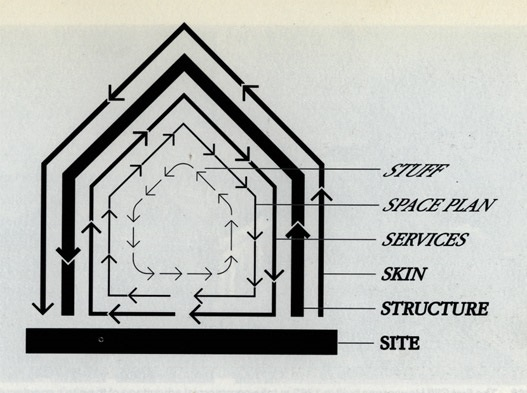
\includegraphics[width=4in]{pictures/brand-diagram}
	\caption[The different layers of change, taken from \cite{brand1995buildings}]
   {The different layers of change \cite{brand1995buildings}}
   \label{brand-diagram}
\end{figure}

The six S's describes the different layers of change, three describing the exterior: Site, Structure and Skin and three describing the interior: Services, Space plan and Stuff.
Each layer has a different rate of change, Site having the longest and Stuff the shortest rate of change, see~\ref{brand-diagram}. As the rate of change differs for the different components of the building, the building is, as Brand notes, constantly `tearing itself apart', or in a more constructive term, constantly evolving.

Brand argues in favor for an approach where the inhabitants of a building can evolve and change the building over time according to their needs \cite{brandBBCvideo}.
He sees this in contrast to a scenario where a single person or group designs a building for others to use.
In light of this, providing inhabitants with higher rates of change could accommodate an even more dynamic relationship between the building and the people living in it.
Inspired by this concept of the building as a living, ever-evolving entity, we want to explore how we can accommodate and design for change in physical interfaces in the context of digital systems in a domestic setting.

Physical interfaces on traditional appliances are generally static and permanent, e.g. buttons on the TV, volume control knob on the stereo, light switches on the wall.
An extra interface layer is often applied here in the form of remote controls - \todo{something something}

We want to explore how physical interfaces can be created on demand in an ad-hoc manner, to better cope with the changes in the buildings space plan and stuff, and better accommodate the changing needs of its inhabitants.
The idea is to let the interface exist when it is needed and then let it slowly perish when it is no longer used, either manually, over time, by natural forces or based on sensory data.

The idea of adding computer systems into the domestic environment is not a new one. An early visual example of the fascination of `smart homes' is seen in the General Motors commercial film \emph{Design for Dreaming} from 1956, where the \emph{Kitchen of the Future} is presented.
Here we see a remote control of the different kitchen appliances, a screen that can show the final result of the recipe it is given, and a seemingly context-aware moving table.
Interestingly three futuristic examples does not fall far from later research done on smart homes, e.g. centralized control of electronics \todo{(ex)}, information appliances \todo{(ex)} and context aware objects\todo{(ex)}.

 \todo{noget kort om Ubicomp}

The domestic setting differs a lot from the traditional office setting where most research on ubiquitous computing has been conducted, and is in some ways even more complex as people in the domestic setting has a lot more freedom as to how they organize their space and time \cite{meyer2003survey}.
Also the aspect of user experience needs special consideration when introducing new technology to the home, whereas in a work setting the user might \emph{need} to use the new technology, imposed upon him by superiors, the technology for the home need to be useable and useful enough so that the user \emph{wants} to use \cite{meyer2003survey}.
A thorough look at the challenges related to creating ubiquitous computing for the home is presented in \cite{edwards2001home}.
Here Edwards et al identifies seven challenges that need to be overcome before the vision of the ubiquitous smart home can become a reality. We will return to these challenges in relation to our own prototypes \todo{ref til prototype sektion}.

Rodden et al. \cite{rodden2003evolution} have built upon Brands framework in the context of ubiquitous computing and the domestic setting and is therefore relevant for us here.
By looking at existing research Rodden et al. identifies three main approaches for creating interactive devices for domestic settings.

\begin{itemize}
  \item \emph{Information Appliance} that are stand-alone, self-contained devices that are often used as a layer of interactive functions on top of an existing appliance.
  \item \emph{Interactive Household Objects} that embeds interactive capabilities into existing household objects to create new means of interaction and communication, often building upon the existing understanding and metaphors associated with the household object.
  \item \emph{Augmented Furniture} that embeds sensory systems into furniture to add interactive capabilities. \ldots
\end{itemize}

Rodden et al. notes that the technology is most intrusive in information appliances, less so in interactive household objects and least in augmented furniture.

\todo{noget om bygninger ikke er nybyggerier}